\documentclass[10pt]{beamer}
\usepackage[utf8]{inputenc}
\usepackage{graphicx}
\usepackage[spanish,mexico]{babel}
\usepackage{amsmath} %simbolos matematicos
\usetheme{Singapore}
\usecolortheme{orchid}
%\useoutertheme{shadow}
%\useinnertheme{rectangles}
\usepackage{multicol}  %texto a varias columnas

\title[Oscilaciones en Sistemas Biológicos: Testosterona]{Oscilaciones en Sistemas Biológicos: Testosterona}
\author{Alejandro Hernández de la Vega\\ César Daniel Rodríguez Rosenblueth \\ Eva Yazmín Santiago Santos}
\institute{Facultad de Ciencias. UNAM} 
\date{}

\begin{document}
\begin{frame}
\titlepage
\end{frame}

\begin{frame}
\frametitle{Índice}
\tableofcontents
\end{frame}

\section{Introducción}

\subsection{Osciladores Biológicos}

\begin{frame}
\frametitle{Osciladores Biológicos}
Su estudio se basa en ecuaciones diferenciales del tipo:

$$\dfrac{du}{dt} = f(u)$$

Donde, para sistemas periódicos se tiene:

$$u(t+T)= (t) $$

con el periodo $T>0$
\end{frame}

\begin{frame}
\frametitle{Osciladores Biológicos}
En algunas ocaciones el sistema está regulado por un control de retroalimentación. \\
$\rightarrow$  Serie de reacciones ligadas
$\rightarrow$ La primera está regulada por una función de retroalimentación.\\

$$ \dfrac{d u_1}{dt} = f(u_n )k_1 u_1 $$ 
$$ \dfrac{d u_r}{dt}= u_{r-1} -k_r u_r $$

con $r=2,3,...,n$ , $ k_r > 0 $ constantes determinadas por el sistema en cuestión y $ f(u)$ la función de retroalimentación.
\end{frame}


\subsection{Testosterona}
\begin{frame}
\frametitle{Testosterona}
\begin{block}{Características}
$\rightarrow$ Es una hormona cuya función principal es estimular el desarrollo de los caracteres sexuales masculinos.\\
$\rightarrow$ Cambios de personalidad relacionados con la concentración de testosterona en la sangre.
\end{block}
\begin{block}{Hombres}
$\rightarrow$ Nivel: 10-35 nanomoles por litro de sangre\\
$\rightarrow$ Oscilan con un periodo de 2 a 3 horas
\end{block}
\begin{block}{Mujeres}
$\rightarrow$ Nivel: 0.7-2.7 nanomoles por litro
\end{block}
\end{frame}

\begin{frame}
\frametitle{Secreción de Testosterona}
Testosterona (T) $\rightarrow$ Hormona Liberadora de Hormona Luteinizante (LHRH) $\rightarrow$ Hormona Luteinizante (LH) $\rightarrow$ Testosterona (T)

Se denota a T, LH y LHRH por $T(t) L(t)$ y $R(t)$ respectivamente.
\end{frame}

\subsection{Comportamiento del Sistema}
\begin{frame}
\frametitle{Comportamiento del Sistema}
\begin{block}{}
Está representado por las siguientes ecuaciones:
$$\frac{dR}{dt} = f(T)-b_{1}R$$
$$\frac{dL}{dt} = g_{1}R-b_{2}L$$
$$ \frac{dT}{dt} = g_{2}L-b_{3}T $$
\end{block}
\begin{block}{}
$b_{1}$, $b_{2}$, $b_{3}$, $g_{1}$, $g_{2}$ son parámetros positivos.\\
$g_{1}$,$g_{2}$ y $f(T)$ son las tasas de secreción\\
$g_{1}$,$g_{2}$ son los valores de prealimentación\\
\end{block}
\end{frame}

\begin{frame}
\frametitle{Puntos de Estabilidad}
Las ecuaciones anteriores tienen sólución en:

$$R_{0} = \frac{f(T_{0})}{b_{1}}$$

$$L_{0} = \frac{b_{3}}{g_{2}}T_{0}$$

Donde $T_{0}>0$ satisface $g_{1}g_{2}f(T_{0}) = b_{1}b_{2}b_{3}T_{0}.$
\end{frame}

\begin{frame}
\frametitle{Puntos de Estabilidad}
Alrededor del punto de equilibrio:

$$ \frac{dx}{dt} = f'(T_{0})z-b_{1}x$$
$$ \frac{dy}{dt} = g_{1}x-b_{2}y $$
$$ \frac{dz}{dt} = g_{2}yt-b_{3}T $$

Donde
$$ z(t)=T(t)-T_{0} $$
$$ y(t)=L(t)-L_{0} $$
$$ x(t)=R(t)-R_{0} $$
\end{frame}

\begin{frame}
\frametitle{Inestabilidad}
Cuando $f'(T_{0}) < 0$ no hay estabilidad: 

(i) si y sólo si 

$$-\frac{g_{1}g_{2}f'(T_{0})}{b_{1}} > \frac{a_{1}a_{2}}{a_{3}}-1$$

Donde:

$$a_{1} = b_{1}+b_{2}+b_{3}$$
$$a_{2}=b_{1}b_{2}+b_{1}b_{3}+b_{2}b_{3}$$
$$a_{3}=b_{1}b_{2}b_{3}$$

(ii) si 

$$-\frac{T_{0}f'(T_{0})}{f(T_{0})} > 8 $$
\end{frame}

\section{Resultados}
\begin{frame}
\begin{center}
 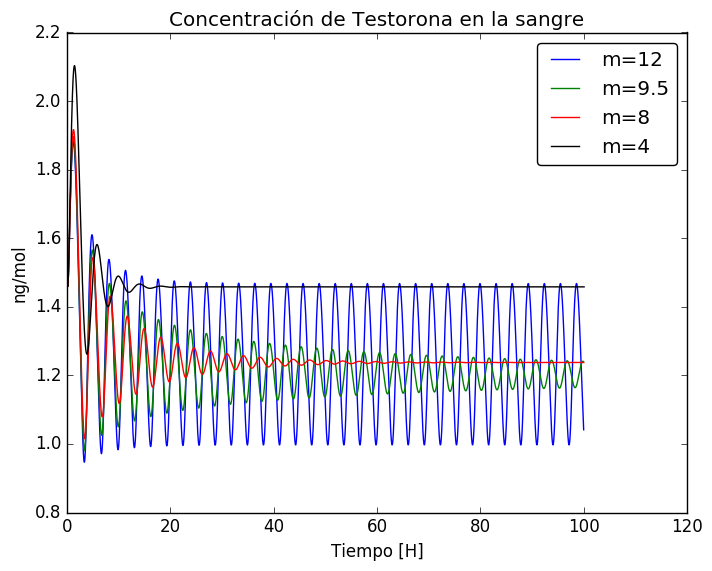
\includegraphics[width=4in]{imagenes/Graficas/testosterona1.png}
\end{center}
\end{frame}

\begin{frame}
\begin{center}
 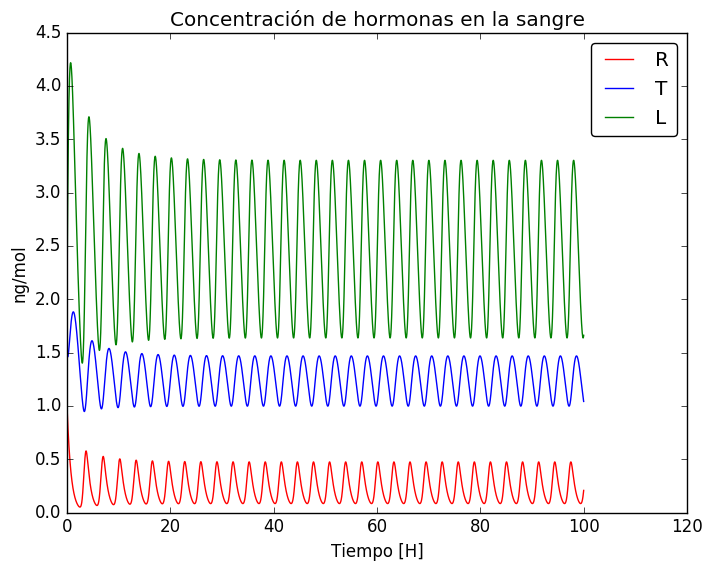
\includegraphics[width=4in]{imagenes/Graficas/hormonas1.png}
\end{center}
\end{frame}

\begin{frame}
\begin{center}
 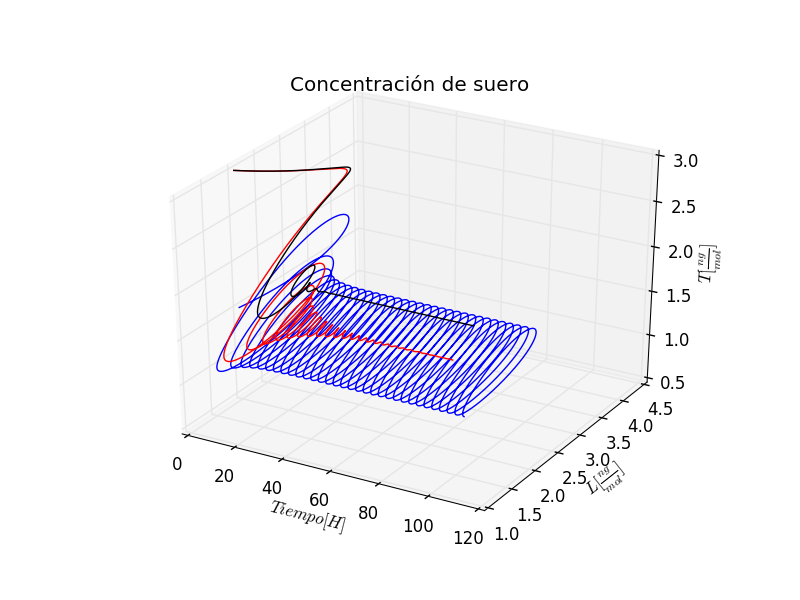
\includegraphics[width=4in]{imagenes/Graficas/g3_3D.png}
\end{center}
\end{frame}


\begin{frame}
\begin{center}
 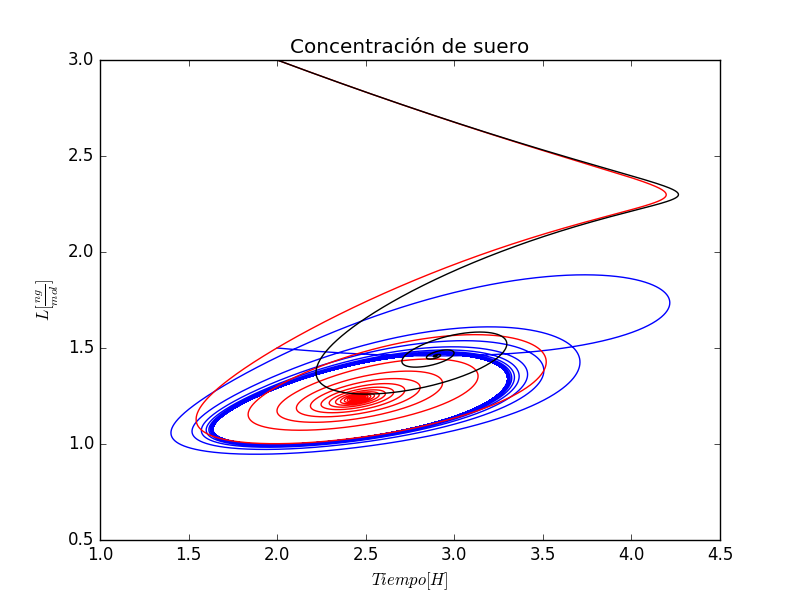
\includegraphics[width=4in]{imagenes/Graficas/g4_2d.png}
\end{center}
\end{frame}

\begin{frame}
\begin{center}
 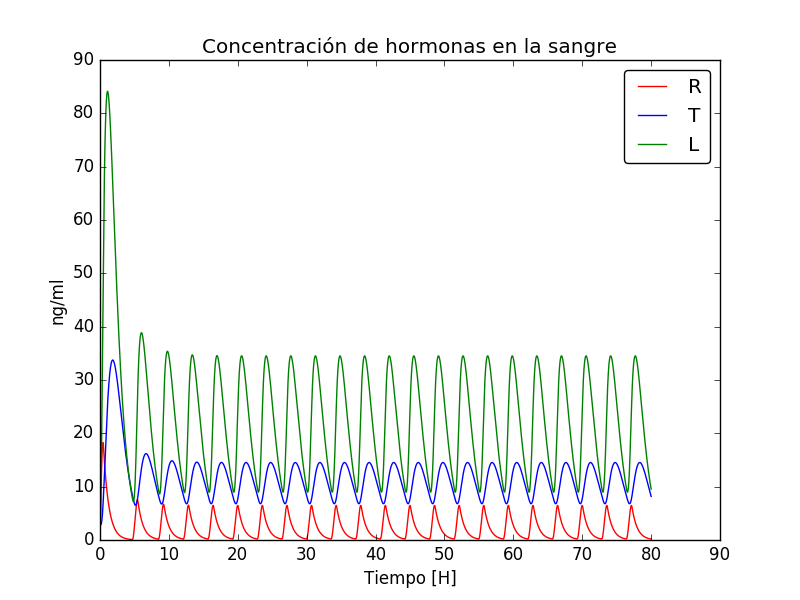
\includegraphics[width=4in]{imagenes/Graficas/g5_g2-modelo2.png}
\end{center}
\end{frame}

\begin{frame}
\begin{center}
 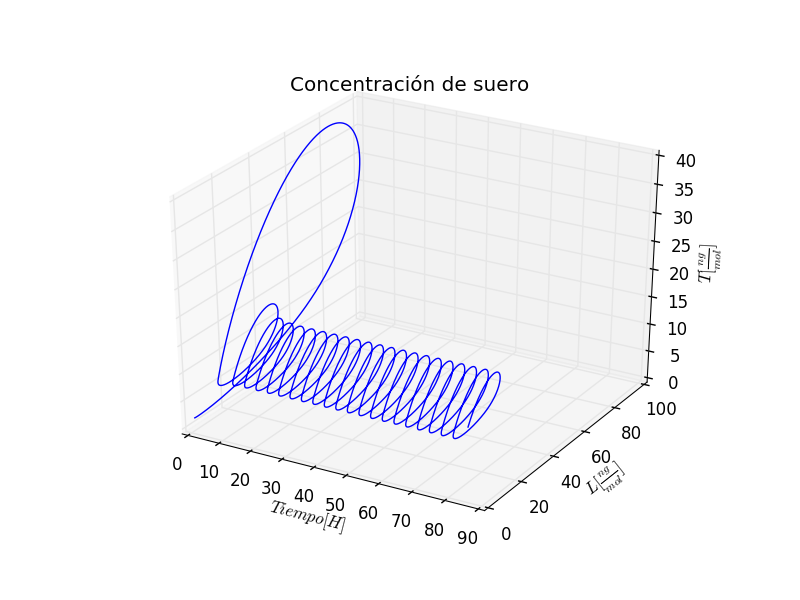
\includegraphics[width=4in]{imagenes/Graficas/g6_modelo2.png}
\end{center}
\end{frame}

\end{document}